\section{Interfacing the LDR through Scilab}
\subsection{Interfacing the LDR}
In this section, we discuss how to carry out the experiments of the
previous section from Scilab. We will list the same two experiments,
in the same order.  The shield has to be attached to the \arduino\ board
before doing these experiments and the \arduino\ needs to be connected to the computer 
with a USB cable, as shown in \figref{arduino}.
The reader should go through the instructions given in
\secref{sec:sci-start} before getting started. 

% In this section, we will explain a few Scilab experiments to read the
% LDR values corresponding to the incident light. The LDR values can be
% read using the following function of Scilab Arduino toolbox:
% \begin{lstlisting}[style=nonumbers]
%   cmd_analog_in(1,port number on Arduino Uno)
% \end{lstlisting}
% where the input argument 1 is fixed for this kit, and the port number corresponds to the analog pin of \arduino that needs to be read.  We will carry out two experiments using Scilab.

\begin{enumerate}
  \item In the first experiment, we will read the LDR values and display it in
        \scilab\ Console. The code for this experiment is 
        given in  \sciref{sci:ldr-read}. As explained earlier in \secref{sec:light-sci}, 
        we begin with serial port initialization. Then, we read the input coming from
        analog pin 5 using the following command:  
        \lstinputlisting[firstline=4,lastline=4]
        {\LocLDRscicode/ldr-read.sce}
        Note that the one leg of the LDR on
        the shield is connected to analog pin 5 of \arduino\, 
        as given in \figref{fig:ldrconn}. The read value is displayed in the 
        \scilab\ Console by the following command: 
        \lstinputlisting[firstline=5,lastline=5]
        {\LocLDRscicode/ldr-read.sce} where {\tt val} contains
        the LDR values ranging from 0 to 1023. If one does the experiment in a completely dark room, the
        reading will be 0. If on the other hand, a bright light, say for instance the torch
        light from mobile, is shined, the value displayed is close to 1023. One will get
        intermediate values by keeping one’s finger on the LDR. To
        encourage the user to have a good hands-on, we run these commands in
        a {\tt for} loop for 50 iterations. While running this experiment, the readers must keep their fingertips on the LDR and
        observe the change in values being printed on the \scilab\ Console. 
        
        
        % We use \sciref{sci:ldr-read} to read the LDR values.  We find the
        %   port number from the computer settings and give it as input to the
        %   {\tt open\_serial} command to start serial port communication. In
        %   our case, the port number is 2. Next, we shall fetch LDR values
        %   using the command, {\tt cmd\_analog\_in}, as explained above. This
        %   is indicated on line 4 of the code. We run this command in a {\tt
        %     for} loop 20 times. In each iteration of the {\tt for} loop, we
        %   acquire LDR data fed to analog pin 5, display it in the Scilab
        %   command window and suspend Scilab operation for 500
        %   milliseconds. The output of this experiment is displayed on the Scilab command
        %   window. After reading the values, we close the serial port using the
        %   command, {\tt close\_serial}, of Scilab-Arduino toolbox.
        
        % \item In this experiment, we will observe the saturation point of LDR,
        %   see \sciref{sci:ldr-led}.  We know that as incident light intensity
        %   increases, voltage at analog input of the \arduino\ board
        %   increases. Thus the ADC values being read by the \arduino\ board also
        %   increase. But after certain high intensity, ADC values reach its
        %   maximum. For 10 bit ADC in Arduino, this high intensity corresponds
        %   to 1023.  Beyond this value, the LDR is incapable of sensing the
        %   change in light intensity and is considered to be saturated. To
        %   observe this saturation point, we can do a simple task of exposing
        %   LDR to high intensity. We can put a torch/light source sensor to
        %   close proximity of LDR.
  \item This experiment is an extension of the previous
        experiment. Here, depending on the resistance of the LDR, we will
        turn the red LED on.  The program for this is available at
        \sciref{sci:ldr-led}.  The value of LDR is read and stored in {\tt
            val}.  In case it is below some threshold (like 300 in \ardref{ard:ldr-led}), 
        it puts a high in pin number 11.  From \secref{sec:led-pril}, 
        one can note that this pin is for the red LED.  If the LDR value is below 300, 
        the red LED will be on, else, it will be turned off.  
        While running this experiment, the readers 
        must keep their fingertips on the LDR so that the threshold is achieved. Accordingly, 
        they can observe whether the red LED is turned on. 
\end{enumerate}

\begin{exercise}
  Carry out the exercise below:
  \begin{enumerate}
    \item Carry out the exercise in the previous section.
    \item Calculate the difference in LDR readings in indoor room
          before lighting the lamp and after lighting the lamp. You can also
          record changes in the room lighting at different times of the day.
  \end{enumerate}
\end{exercise}

\subsection{Scilab Code}
\label{sec:ldr-scilab-code}
\addtocontents{cod}{\protect\addvspace{\codclr}}

\begin{scicode}
  \ccaption{Read and display the LDR values}
  {Read and display the LDR values.  Available at
    \LocLDRscibrief{ldr-read.sce}.}
  \label{sci:ldr-read}
  \lstinputlisting{\LocLDRscicode/ldr-read.sce}
\end{scicode}

\begin{scicode}
  \ccaption{Turning the red LED on and off}
  {Turning the red LED on and off.  Available at
    \LocLDRscibrief{ldr-led.sce}.}
  \label{sci:ldr-led}
  \lstinputlisting{\LocLDRscicode/ldr-led.sce}
\end{scicode}

\section{Interfacing the LDR through Xcos}
Next, we shall perform the above mentioned experiments, to read LDR
values, through Xcos.  We will carry out the same two experiments as in the previous
sections.  For each, will give the location
of the zcos file and the parameters to set.  The reader should go
through the instructions given in \secref{sec:xcos-start} before
getting started.

\begin{enumerate}
  \item First we will read the LDR values and display it.  When the
        file required for this experiment is invoked, one gets the GUI as in
        \figref{fig:ldr-read}.  In the caption of this figure, one
        can see where to locate the file. 
        
        As discussed in earlier chapters, we start with the initialization
        of the serial port. Next, using {\tt Analog Read} block, we read
        the values of LDR connected on analog pin 5. Next, we use a scope to plot the values 
        coming from this pin. When this Xcos file is simulated, a plot is opened, 
        as shown in \figref{fig:ldr-read-plot}. 
        
        \begin{figure}
          \centering
          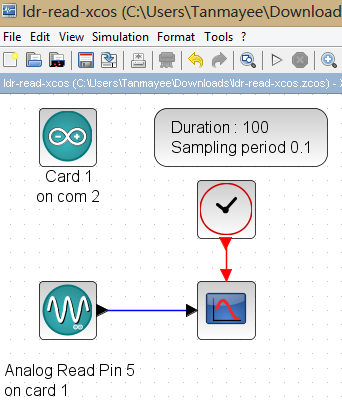
\includegraphics[width=\smfig]{\LocLDRfig/ldr-read-xcos.PNG}
          \caption[Xcos diagram to read LDR values]{Xcos diagram to read LDR
            values.  
            This is what one sees when 
            \LocLDRscibrief{ldr-read.zcos}, is invoked.}
          \label{fig:ldr-read}
        \end{figure}
        
        \begin{figure}
          \centering
          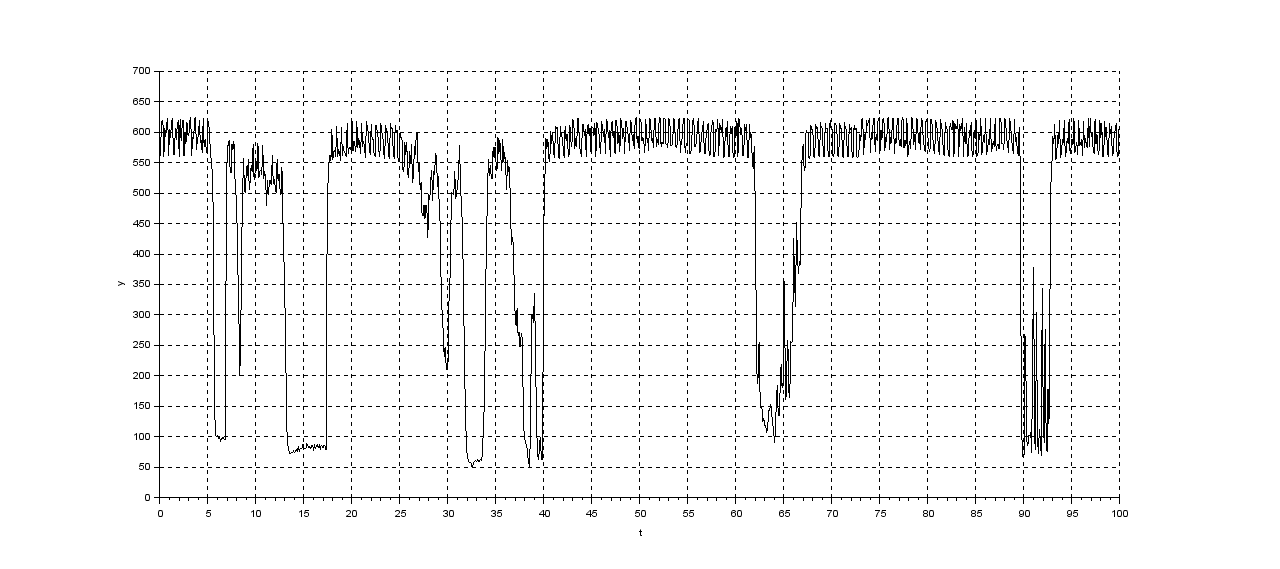
\includegraphics[width=\hgfig]{\LocLDRfig/ldr-read-plot.PNG}
          \caption{Plot window in Xcos to read LDR values}
          \label{fig:ldr-read-plot}
        \end{figure}
        
        We will next explain how to set the parameters for this simulation.
        To set value on any block, one needs to right click and open the
          {\tt Block Parameters} or double click.  The values for each block
        is tabulated in \tabref{tab:ldr-read}.  All other parameters are to
        be left unchanged.
        \begin{table}
          \centering
          \caption{Xcos parameters to read LDR}
          \label{tab:ldr-read}
          \begin{tabular}{llc} \hline
            Name of the block & Parameter name             & Value     \\ \hline
            ARDUINO\_SETUP    & Identifier of Arduino Card & 1         \\
                              & Serial com port number     & 2\portcmd \\ \hline
            TIME\_SAMPLE      & Duration of acquisition(s) & 10        \\
                              & Sampling period(s)         & 0.1       \\ \hline
            ANALOG\_READ\_SB  & Analog Pin                 & 5         \\
                              & Arduino card number        & 1         \\ \hline
            CSCOPE            & Ymin                       & 0         \\ 
                              & Ymax                       & 1023      \\
                              & Refresh period             & 100       \\ \hline
            CLOCK\_c          & Period                     & 0.1       \\
                              & Initialisation Time        & 0         \\ \hline
          \end{tabular}
        \end{table}
        
        During this experiment, we vary the light incident on LDR by using
        light sources and obstacles such as torch light, paper,
        hand (or fingertips), etc. and observe the LDR readings in the plot, as shown in 
        \figref{fig:ldr-read-plot}. We observe that with a constant light source, the LDR output saturates after some time. 
        %The output for this experiment is shown in \figref{fig:ldrsatout}.
        
        %   \begin{figure}
        %     \centering
        %     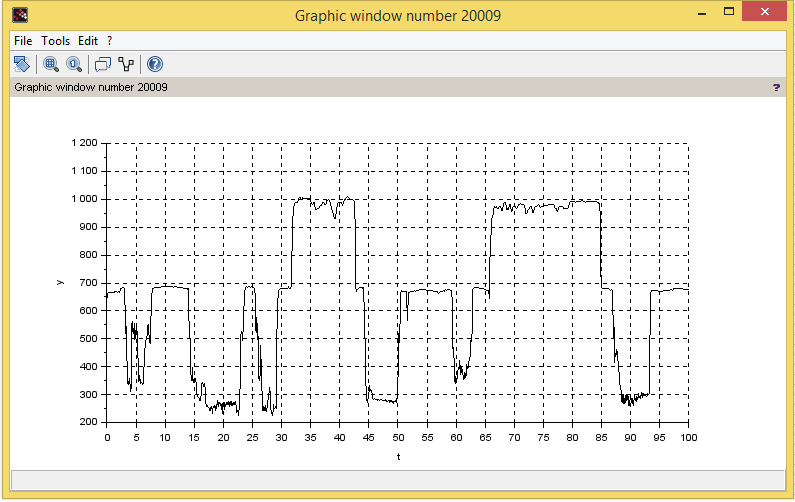
\includegraphics[width=\lgfig]{\LocLDRfig/ldr-sat-out.png}
        %     \caption[LDR output for varying intensity of incident light, as
        %     seen in Xcos] {LDR output for varying intensity of
        %       incident light, as seen in Xcos.  This is what one sees when
        %       {\tt \LocLDRscibrief/ldr-read-xcos.zcos} is invoked.}
        %     \label{fig:ldrsatout}
        %   \end{figure}
        
  \item In the second experiment, we take a step further and control the
        state of red LED in accordance with the LDR values. When the file required for this
        experiment is invoked, one gets the GUI as in \figref{fig:ldr-led}.
        In the caption of this figure, one can see where to locate the file.
        
        \begin{figure}
          \centering
          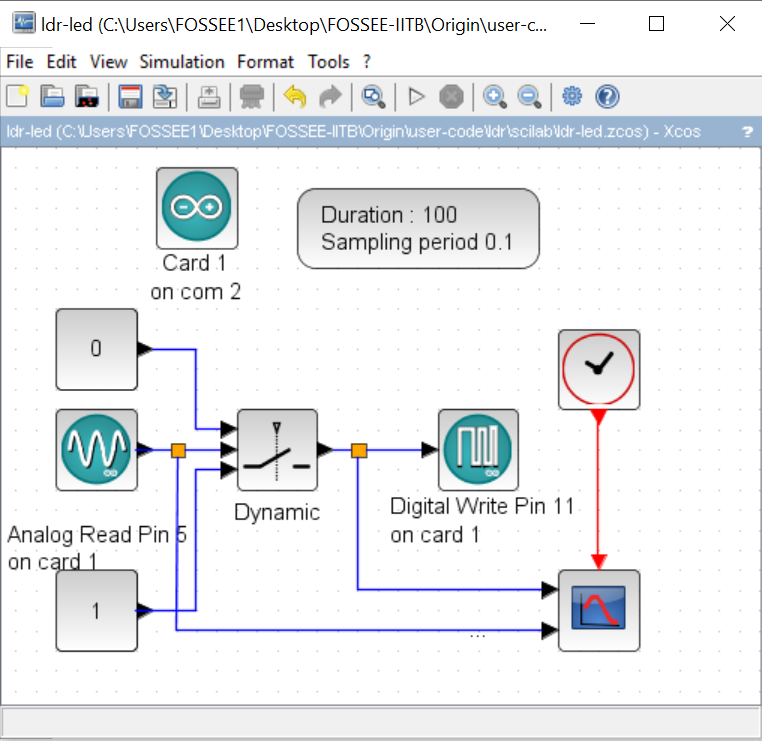
\includegraphics[width=\lgfig]{\LocLDRfig/ldr-led-2.png}
          %    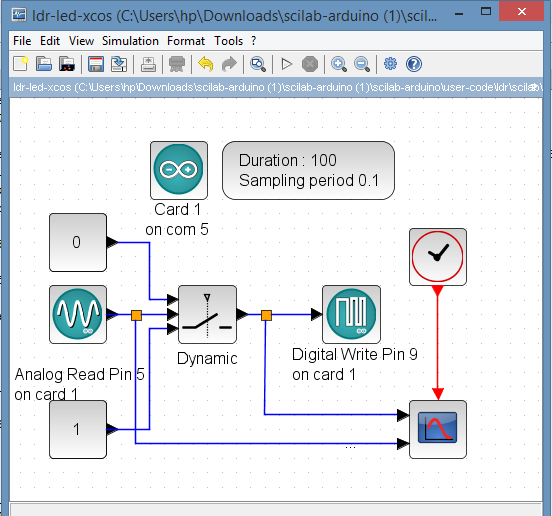
\includegraphics[width=\smfig]{\LocLDRfig/ldr-led-xcos.PNG}
          \caption[Xcos diagram to read the value of the LDR, which is used
            to turn the blue LED on or off] {Xcos diagram to read the value of
            the LDR, which is used to turn the blue LED on or off.  This is
            what one sees when \LocLDRscibrief{ldr-led-xcos.zcos}, is
            invoked.}
          \label{fig:ldr-led}
        \end{figure}
        
        We will next explain how to set the parameters for this simulation.
        To set value on any block, one needs to right click and open the
          {\tt Block Parameters} or double click.  The values for each block
        is tabulated in \tabref{tab:ldr-led}.  In the CSCOPE\_c block, the
        two values correspond to two graphs, one for digital write and other
        for analog read values. All other parameters are to be left
        unchanged. When this Xcos file is simulated, a plot is opened, 
        as shown in \figref{fig:ldr-led-read-plot}. 
        
        \begin{figure}
          \centering
          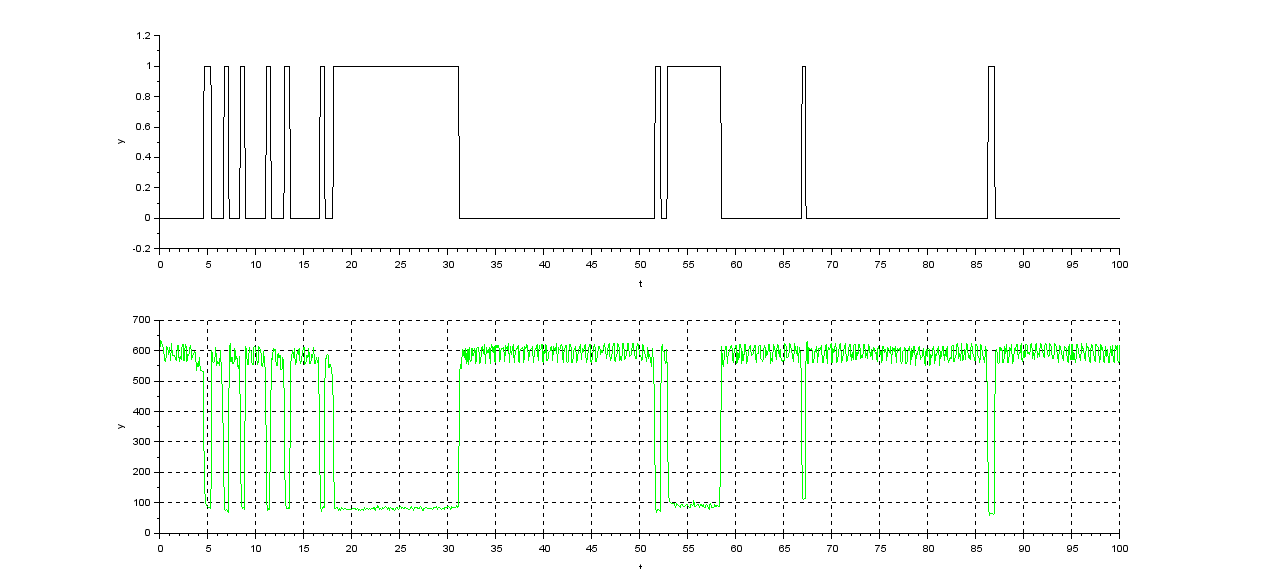
\includegraphics[width=\hgfig]{\LocLDRfig/ldr-led-read-plot.PNG}
          \caption{Plot window in Xcos to read LDR values and the state of LED}
          \label{fig:ldr-led-read-plot}
        \end{figure}
        
        \begin{table}
          \centering
          \caption{Xcos parameters to read LDR and regulate blue LED}
          \label{tab:ldr-led}
          \begin{tabular}{llc} \hline
            Name of the block  & Parameter name             & Value     \\ \hline
            ARDUINO\_SETUP     & Identifier of Arduino Card & 1         \\
                               & Serial com port number     & 2\portcmd \\ \hline
            TIME\_SAMPLE       & Duration of acquisition(s) & 10        \\
                               & Sampling period(s)         & 0.1       \\ \hline
            ANALOG\_READ\_SB   & Analog pin                 & 5         \\
                               & Arduino card number        & 1         \\ \hline
            CMSCOPE            & Ymin                       & 0 0       \\ 
                               & Ymax                       & 1 1023    \\
                               & Refresh period             & 100 100   \\ \hline
            CLOCK\_c           & Period                     & 0.1       \\
                               & Initialisation time        & 0         \\ \hline
            SWITCH2\_m         & Datatype                   & 1         \\
                               & threshold                  & 300       \\
                               & pass first input if field  & 0         \\
                               & use zero crossing          & 1         \\ \hline
            DIGITAL\_WRITE\_SB & Digital pin                & 9         \\
                               & Arduino card number        & 1         \\ \hline
          \end{tabular}
        \end{table}
\end{enumerate}

